\section{PyTorch}
\subsection{Overview}
PyTorch \cite{Paszke2017} is a popular ML framework with a Python frontend (as well as others).
Its key features include:
\begin{itemize}[topsep=0.2em, parsep=0.5\parskip]
    \item Easily execute tensor computations in Python, with an API similar to the Numpy library \cite{VanDerWalt2011}.
    \item Easily transfer between PyTorch tensors and Numpy nd-arrays.
    \item Easily accelerate these computations on a GPU.
    \item Easily evaluate derivates of the computation with respect to the tensors involved.
    The user simply tells PyTorch to track the gradients when constructing a tensor.
    \item \textit{Define-by-run} execution: The user does not need to statically define a computation graph like in TensorFlow \cite{tensorflow2015-whitepaper}, even when taking derivatives.
    They can execute any computation using native Python constructs such as control flow.
    \item Provides a rich API for constructing common ML operators, such as convolutions or ReLU
    \item Allows the user to extend the API with their own operators.
    Can easily interleave pre-defined and custom operators in one computation.
    \item Provides distribution strategies for further scaling out ML training and inference.
\end{itemize}

An example PyTorch program that demonstrates some of these features is given in Listing \ref{lst:2-example-pytorch}.


\vfill

\begin{listing}[H]
    \inputminted[
        frame=lines,
        framesep=2mm,
        baselinestretch=1.2,
        fontsize=\footnotesize,
        linenos,
        style=perldoc
    ]{python}{listings/pytorch_demo.py}
    \caption{Example PyTorch program}
    \label{lst:2-example-pytorch}
\end{listing}

\subsection{Autograd}
PyTorch's Autograd module is responsible for the evaluation of derivates of dynamically defined computations.
It uses true reverse-mode automatic differentation.
That is, the user runs their forward computation normally and it is automatically augmented with a backwards graph.
As stated above, this means there is no need to define a static graph, and native Python control flow can be used.

Consider, in Figure \ref{fig:2-autograd-graph}, some PyTorch code and the backward graph generated by Autograd.
It is very important to point out that this graph, nor the following explanation of how it is constructed, do not exactly correspond to how Autograd is implemented; only to help convey the ideas at a high level.

\begin{figure}[H]
    \begin{minipage}{0.4\textwidth}
        \centering
        \inputminted[
            frame=lines,
            framesep=2mm,
            %baselinestretch=1.2,
            fontsize=\footnotesize,
            style=perldoc
        ]{python}{listings/autograd_demo.py}
        %\captionof{listing}{PyTorch forward code.}
    \end{minipage}
    \begin{minipage}{0.6\textwidth}
     \centering
     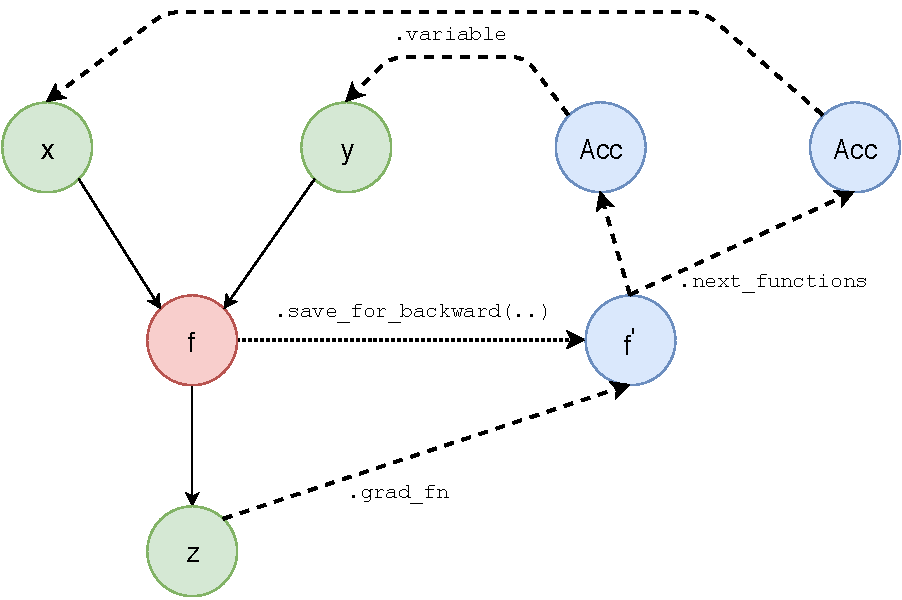
\includegraphics[width=\linewidth]{autograd_graph.pdf}
     %\captionof{listing}{Another sub caption}
    \end{minipage}
    %\captionof{listing}{SomeCaption}
    \caption{Forward PyTorch code and its autograd backwards graph. Green nodes are tensors. Red nodes are forward functions. Blue nodes are backward functions. Dashed edges are object composition (fields of the object). Dotted edges are function calls. Straight edges represent the forward computation.}
    \label{fig:2-autograd-graph}
\end{figure}

First, \texttt{x} and \texttt{y} are constructed with \texttt{requires\_grad=True},
 telling Autograd to build a backward graph on computations that use them.
They will also have \texttt{is\_leaf=True} as they were explicitly set to a value by the user, rather than being constructed from existing tensors.
When \texttt{z} is constructed by applying the operator \texttt{f} to \texttt{x} and \texttt{y}, Autograd sees that \texttt{x} and \texttt{y} require gradient.
This results in a number of steps occuring:
\begin{enumerate}[topsep=0.1em]
    \item \texttt{z} will require gradient.
    \item \texttt{z.grad\_fn} will be set to the corresponding backward operator of \texttt{f}, which will be denoted \texttt{f'}.
    \item \texttt{f} will save handles to any tensors \texttt{f'} requires for the backwards pass, such as its inputs in the case of multiplication.
    \item \texttt{f'.next\_functions} will be set to point to the \texttt{.grad\_fn}s of \texttt{x} and \texttt{y}.
    \item However, because they are leaves, actually \texttt{AccumulateGrad} backward functions will be constructed for each of them instead.
    These accumulate all incoming upstream gradients into \texttt{.grad} of their tensor so the user can access it after the backwards pass is complete.
\end{enumerate}
Because \texttt{z} requires gradient and has its \texttt{.grad\_fn} set, when subsequent operators are applied to it, the exact same process will occur, extending the backward graph.
Thus, any time an operation is performed, the backward graph is being dynamically constructed alongside.
This is why no static graph is required beforehand.

There is no forward graph during this process.
The straight edges of Figure \ref{fig:2-autograd-graph} represent the computation that occurs; there are no pointers between the objects.

Finally, when the user calls \texttt{.backward()} on the output tensor, the backward graph already in place will be traversed.
An Autograd backward function takes upstream gradients for each of its outputs and produces downstream gradients for each of its inputs that require gradient, possibly using outputs saved from the forward pass.
The gradients are then propagated downstream using the backward function's \texttt{.next\_functions}.
The process bottoms-out when this field is empty, usually when an \texttt{AccumulateGrad} for a leaf tensor has been reached.
These accumulate the incoming upstream gradients into the tensor in their \texttt{.variable} field.

One thing to consider is mutations to the tensors.
If a tensor is mutated after a computation is run and the backward graph defined, the backward function no longer has access to the tensor originally involved in the forward, because it only stored a handle to the tensor object, it did not make a copy of the data. 
Thus, though tensors are mutable in PyTorch, they will invalidate existing backward graphs involving that tensor, causing an error to be thrown if the user attempts to traverse that graph.

It can also be useful to detach tensors from the backward graph. Calling \texttt{.detach()} on a tensor will create a new tensor object (aliasing the same data) that is not part of the Autograd graph.
The new tensor will be a leaf and does not require gradient.
When the original backward graph is traversed, the new tensor will not have a \texttt{.grad\_fn} that is invoked.

Detaching is often used to ensure the backward graph is cleared from memory when the backward pass has been done and the gradients are no longer required, but we would like to keep a forward tensor.
I will use detaching in my implementation of checkpointing with multiple recomputations to manually control how execution moves forward and backward along a sequence.
%More on this in \todo{[sec]}.

For a more in-depth look on Autograd internals, I recommend starting with Elliot Waite's excellent tutorial on Youtube \footnote{\url{https://youtu.be/MswxJw-8PvE}, accessed 26/08/19}.

%\todo{add extra stuff if required}
%TODO: Define an autograd function in code.
%TODO: Defining a module using function
%TODO: Possibly show a standard training loop, if can be made terse enough.
